%==============================================================================
% Importando a classe
%==============================================================================
\documentclass{templufla}          


%==============================================================================
% Configuração dos pacotes necessários
%==============================================================================
% Primeiros pacotes (alguns precisam ser importados depois)

% TEXTOS
\usepackage[brazil]{babel}       % hifenização e títulos em português do Brasil
\usepackage[T1]{fontenc}         % usa fontes postscript com acentos
\usepackage[utf8]{inputenc}      % permite edição direta com acentos
\usepackage{listings}            % para inserção de código
\usepackage{fancyvrb}            % para inserção de saídas de comandos

% MATEMÁTICA
\usepackage{amsmath}             % pacote da AMS para Matemática Avançada
\usepackage{amssymb}             % símbolos extras da AMS
\usepackage{mathtools}			 % para mais comandos de matemática
\usepackage{latexsym}            % símbolos extras do LaTeX

% TABELAS
\usepackage{longtable}           % para tabelas muito grandes
\usepackage{array}               % para mais opções em tabelas
\usepackage{colortbl}            % para cores em tabelas
\usepackage{multirow}            % para células com várias linhas
\usepackage{multicol}            % para células com várias colunas

% FIGUAS E GRÁFICOS
\usepackage{xcolor}              % para mais cores
\usepackage{subfigure}           % para figuras dentro de figuras
\usepackage{caption}             % para remodelar o formato dos títulos
% Impede que uma figura "escape" para outra seção (opcional: só é usado se o
% pacote estiver disponível na distribuição TeX, como no Overleaf).
\IfFileExists{placeins.sty}{\usepackage[section]{placeins}}{}

%==============================================================================
% Posicionamento dos elementos flutuantes (figuras)
% Os parâmetros padrão do LaTeX são restritivos e empurram figuras grandes para
% páginas distantes do ponto em que são citadas. Os valores abaixo permitem que
% uma figura ocupe boa parte do topo (ou do rodapé) da página em que aparece,
% mantendo-a próxima do texto que a explica.
\setcounter{topnumber}{2}          % até 2 figuras no topo da página
\setcounter{bottomnumber}{2}       % até 2 figuras no rodapé da página
\setcounter{totalnumber}{3}        % até 3 figuras por página
\renewcommand{\topfraction}{0.85}      % fração máxima da página ocupada no topo
\renewcommand{\bottomfraction}{0.70}   % fração máxima da página ocupada no rodapé
\renewcommand{\textfraction}{0.10}     % fração mínima de texto por página
\renewcommand{\floatpagefraction}{0.80}% ocupação mínima de uma página só de figuras

%==============================================================================
% O pacote hyperref para referência cruzadas dentro do documento \ref e \autoref

% Setspace precisa estar antes do hyperref para usar a versão atual do abntex.
\usepackage{setspace}

% Definindo cores para os links cruzados
\definecolor{rltred}{rgb}{0.2,0,0}
\definecolor{rltgreen}{rgb}{0,0.2,0}
\definecolor{rltblue}{rgb}{0,0,0.2}


% Importa hyperref
\usepackage[%
hidelinks, % colorlinks=true, | Troque se quiser link com cor
urlcolor=rltblue,       % \href{...}{...} external (URL)
filecolor=rltgreen,     % \href{...} local file
linkcolor=rltred,       % \ref{...} and \pageref{...}
citecolor=rltgreen,%
]{hyperref} % 


%==============================================================================
% Citações/referências no formato ABNT, utilizando o pacote abntex2.
% O pacote já vem na maioria das distribuições (texLive, MikTeX, Overleaf e etc...)
% mas, caso você seja super roots e não use os listados, precisa instalar o abntex2:
% http://abntex.codigolivre.org.br/

% A versão disponível com esse template sofreu algumas alterações para se adaptar ao
% padrão atual, já que a original está desatualizada.
% Para mais informações, vizite o repositório oficial do template.


% abnt-emphasize=bf coloca o título das bibliografias em negrito
% abnt-etal-list=3 limita o número de autores antes de et al. para 3
% abnt-url-package=xurl diz para usar o pacote xurl
\usepackage[alf, abnt-etal-list=3, abnt-url-package=xurl, abnt-emphasize=bf]{abntex2cite}

%==============================================================================
% Ajustando os pacotes importados

% Definindo cores para elementos tabulares
\newcolumntype{Z}{|>{\columncolor[gray]{0.9}}l|} %cor cinza em células
\newcolumntype{L}[1]{>{\raggedright\let\newline\\\arraybackslash\hspace{0pt}}m{#1}}
\newcolumntype{C}[1]{>{\centering\let\newline\\\arraybackslash\hspace{0pt}}m{#1}}
\newcolumntype{R}[1]{>{\raggedleft\let\newline\\\arraybackslash\hspace{0pt}}m{#1}}

% Definindo espaçamento vertical de elementos tabulares
\renewcommand{\arraystretch}{1.5}

% Configuração padrão do listings (ambiente de código)
\lstset{
	extendedchars=true,
	breaklines=true,
	tabsize=3,
	basicstyle=\linespread{1}\ttfamily\normalsize,
	stringstyle=\em,
	showstringspaces=true,
	inputencoding=utf8,
	captionpos=t,
	backgroundcolor=\color{black!5},
	literate={{á}{{\'a}}1 {é}{{\'e}}1 {í}{{\'i}}1 {ó}{{\'o}}1 {ú}{{\'u}}1
	{Á}{{\'A}}1 {É}{{\'E}}1 {Í}{{\'I}}1 {Ó}{{\'O}}1 {Ú}{{\'U}}1
	{â}{{\^a}}1 {ê}{{\^e}}1 {ô}{{\^o}}1
	{Â}{{\^A}}1 {Ê}{{\^E}}1 {Ô}{{\^O}}1
	{ã}{{\~a}}1 {õ}{{\~o}}1 {ẽ}{{\~e}}1 
	{ç}{{\c{c}}}1
	{à}{{\`{a}}}1{À}{{\`{A}}}1}
}

% Ajustes adicionais do listings: numeração de linhas, moldura e palavras-chave
\renewcommand{\lstlistingname}{Código}
\lstset{
	numbers=left,
	numberstyle=\tiny,
	numbersep=8pt,
	frame=single,
	framesep=4pt,
	keywordstyle=\bfseries,
	morekeywords={const,let,var,function,return,if,else,async,await,import,
		export,from,interface,type,for,of,new,true,false,null,this,class}
}

% Pacote para diagramas (arquitetura e fluxos)
\usepackage{tikz}
\usetikzlibrary{shapes.geometric, arrows.meta, positioning, fit, calc}

% Destaque de alteracoes para revisao do orientador.
% \destacartrue gera a versao com marcacao amarela (para revisao do orientador);
% \destacarfalse gera a versao limpa (final).
\newif\ifdestacar
\destacarfalse

% \novo{...} para trechos inline (quebra com o texto, usando texto em negrito laranja).
% \novop{...} para paragrafos inteiros (com fundo amarelo).
% O recuo de primeira linha e preservado dentro da caixa amarela, para que o
% paragrafo destacado fique alinhado como os demais paragrafos do texto.
\newlength{\recuonovop}
\AtBeginDocument{\setlength{\recuonovop}{\parindent}}
\newcommand{\novo}[1]{\ifdestacar{\textcolor{orange!90!black}{\textbf{#1}}}\else{#1}\fi}
\newcommand{\novop}[1]{\ifdestacar
  \par\noindent\colorbox{yellow!50}{\begin{minipage}{\dimexpr\linewidth-2\fboxsep\relax}%
  \setlength{\parindent}{\recuonovop}\indent #1\end{minipage}}\par\vspace{4pt}
  \else
  \par #1\par
  \fi}
\newcommand{\novamarca}[1]{\ifdestacar{\par\noindent\textcolor{orange!80!black}{\textbf{[ALTERADO: #1]}}\par}\else\fi}

% Carregamento do glossário, listas de siglas, símbolos e etc
\loadglsentries{glossarios/abreviaturas}
\loadglsentries{glossarios/glossario}
\loadglsentries{glossarios/siglas}
\loadglsentries{glossarios/simbolos}

% Especificando hifenizações que por ventura LaTeX não saiba fazer
% Por padrão 99,9% dos termos em português devem ser hifenizados corretamente.
% Adicione aqui palavras precise especificar como hifenizar (ou não hifenizar)
\hyphenation{software am-bien-te coor-de-na-ção FAE-PE TelEduc Williams UFLA Murray Bookchin}

% Adaptando os nomes das seções
% Também pode ser usado para alterar a lingua dos elementos
% (ex Figura para Figure, caso seu texto esteja em inglês).
\addto\captionsbrazil{
	\renewcommand{\chaptername}{Seção}
	\renewcommand{\subsectionname}{Seção}
	\renewcommand{\subsubsectionname}{Seção}
	%\renewcommand{\figurename}{Figure}
}
\addto\extrasbrazil{
	\renewcommand{\chapterautorefname}{Seção}
	\renewcommand{\subsectionautorefname}{Seção}
	\renewcommand{\subsubsectionautorefname}{Seção}
	%\renewcommand{\figureautorefname}{Figure}
}


%==============================================================================
% Dados da monografia, capa: autor, titulo, banca, etc... - SUBSTITUA DE ACORDO
%==============================================================================
% Dados para o arquivo PDF (metadados)
\hypersetup{%
% Titulo
pdftitle={Relatório Técnico de Desenvolvimento de Aplicações Web na Empresa Zeeway},
% Autor
pdfauthor={Lucas Henrique Lopes Costa},
% Descrição
pdfsubject={Relatório Técnico de Desenvolvimento de Aplicações Web na Empresa Zeeway.},
% Palavras-Chave
pdfkeywords={desenvolvimento web; React; TypeScript; Scrum; agronegócio.}
}
	
%==============================================================================
% Informações básicas

% Nome da(s)/do(s) autora(s)/autor(es)
\author{Lucas Henrique Lopes Costa}

% Título do trabalho, em lígua vernácula
\title{Relatório Técnico de Desenvolvimento de Aplicações Web na Empresa Zeeway}

% Subítulo do trabalho, em lígua vernácula
% \subtitle{}

% Edição, se houver. Caso contrário, comente.
% \edicao{}

% Data de publicação
\date{2026}

% Tipo do Documento
\tipo{Relatório técnico apresentada à Universidade Federal de Lavras, como parte das exigências do programa de Graduação em Sistemas de informação, para a obtenção do título de Bacharel em Sistema de Informação}


% Orientador/orientadora
% Altere o comando para os diferentes gêneros
\orientador{Prof. Paulo Afonso Parreira Júnior}
%\orientadora{Profa. [Nome da Orientadora]}

% Coorientador/coorientadora - Comente se não houver.
%\coorientador{Prof. [Nome do Coorientador]}

% Local
\local{Lavras -- MG}

%==============================================================================
% Informações da banca

% Membros da banca. Até quatro membros. 
% Deve ser {nome}{instituição}.
% Comente os últimos se a banca tiver menos membros.
% \bancaum{Prof. [Nome Banca Um]}{UFLA}
% \bancadois{Prof. [Nome Banca Dois]}{UFLA}
%\bancatres{}{}
%\bancaquatro{}{}

% Data da defesa
\defesa{\_\_\_\_\_\_\_\_ de \_\_\_\_\_\_\_\_ de \_\_\_\_\_\_\_\_\_\_\_\_\_\_}

%==============================================================================
% Dados para Ficha catalográfica, gerada pelo sistema da Biblioteca da UFLA
% http://www.biblioteca.ufla.br/FichaCatalografica/
% dados para ficha catalográfica

% Texto acima da ficha
\preparofichacat{Ficha catalográfica elaborada pela Coordenadoria de Processos Técnicos da Biblioteca Universitária da UFLA, com dados informados pelo(a) próprio(a) autor(a).}

% Primeiro autor - como na primeira linha da ficha catalográfica
\fcautor{Costa, Lucas Henrique Lopes}

% Autores, separados por vírgula
\fcautores{Lucas Henrique Lopes Costa}

% Caso trabalho seja ilustrado
\fcilustrado{il.}

% Tipo do trabalho
\fctipo{Trabalho de Conclusão de Curso (graduação)}

% Preencher com os dados gerados pelo sistema da Biblioteca da UFLA
\fccatalogacao{1. Desenvolvimento web. 2. React. 3. TypeScript. 4. Scrum. I. Universidade Federal de Lavras. II. Título.}
\fcclasi{[Número de Classificação]}

%==============================================================================
% Se vc já defendeu e tem o arquivo escaneado da folha de rosto, 
% descomente e altere o nome do arquivo
%\folhaAprovacaoAssinada{folharosto}


%==============================================================================
% O documento em si
%==============================================================================
\begin{document}

%==============================================================================
%Elementos pré-textuais

% Cria capa, folha de rosto, folha de aprovação e ficha
\maketitle

% Dedicatória
\dedic{Dedico este trabalho a Deus, que guiou os meus passos. Aos meus pais, Lidiana e Antônio, ao meu irmão Marcos Túlio, e a toda a minha família, que sempre me deram apoio para chegar onde estou.}

% Agradecimentos
\thanks{
Agradeço primeiramente a Deus, por me dar saúde, resiliência e por guiar os meus passos ao longo de toda esta jornada universitária.

Aos meus pais, Lidiana e Antônio, e ao meu irmão, Marcos Túlio, o meu muito obrigado por serem a minha base. Gratidão pelo apoio incondicional de vocês.

Um agradecimento muito especial aos meus avós, Maria Aparecida e Waldeli; e meus padrinhos, Alessandra e Hélio, por todo o incentivo. Às minhas primas de coração, Fernanda, Júlia e Laura, agradeço por estarem sempre ao meu lado, me acompanhando e se preocupando comigo em cada etapa desse processo. Ao meus tios, Kelson, Ana, Kerley, por também estarem comigo nessa trajetória.

Gostaria de expressar minha profunda gratidão ao Luiz Fernando e ao seu pai, José Ari Ferreira. Vocês foram as pessoas que me motivaram a vir para a UFLA, que me deram a primeira grande oportunidade de trabalho e que acreditaram em mim. Tenho um enorme carinho e uma gratidão imensa por tudo o que construímos e vivemos juntos na Zeeway.

Por fim, agradeço ao professor Paulo Afonso pela orientação, paciência e por compartilhar sua experiência para a construção deste trabalho, e a todos os professores do curso que contribuíram para a minha formação profissional e pessoal.}

% Resumo e palavras-chave
% As palavras-chave PRECISAM vir primeiro
\palchaves{desenvolvimento web; React; TypeScript; Scrum; agronegócio.}
\resumo{%
Este trabalho apresenta as atividades desenvolvidas durante o estágio supervisionado na empresa Zeeway, sediada em Lavras (MG), no desenvolvimento de uma plataforma web sob demanda para uma empresa de pesquisa agrícola de Lavras, atuante no agronegócio e especializada em análises de solos e sementes. A atuação concentrou-se na construção da camada de interface (\textit{front-end}) da plataforma, responsável pelo registro e pela análise dos protocolos de pesquisa, em substituição ao uso descentralizado de planilhas. As tecnologias adotadas foram o \textit{React} e o \textit{TypeScript}, com componentes do \textit{Material UI}, formulários com \textit{Formik} e \textit{Yup}, gerenciamento de estado global com \textit{Zustand}, comunicação com a API por meio de \textit{Axios} e \textit{React Query}, e visualização de dados com \textit{ApexCharts}. O desenvolvimento foi conduzido pela metodologia ágil \textit{Scrum}, com \textit{Sprints} quinzenais. As atividades incluíram a autenticação com \textit{JSON Web Tokens} (JWT) e a renovação automática do \textit{token}, o controle de acesso por perfil no nível das rotas, formulários extensos com validação declarativa, a geração automatizada de gráficos e \textit{dashboards} e a exportação de imagens com a identidade visual do cliente. A experiência consolidou competências em desenvolvimento web e em visualização de dados, e permitiu vivenciar a engenharia de \textit{software} em equipe, com cliente externo e regras de negócio reais.
}

% Abstract e keywords
% As keywords PRECISAM vir primeiro
\keywords{web development; React; TypeScript; Scrum; agribusiness.}
\abstract{%
This report presents the activities developed during the supervised internship at Zeeway, a company based in Lavras (MG), in the development of a custom web platform for an agricultural research company also based in Lavras, working in the agribusiness sector and specialized in soil and seed analysis. The work focused on building the front-end layer of the platform, responsible for registering and analyzing research protocols, replacing the decentralized use of spreadsheets. The technologies adopted were React and TypeScript, with Material UI components, forms with Formik and Yup, global state management with Zustand, API communication through Axios and React Query, and data visualization with ApexCharts. The development followed the Scrum agile methodology, with biweekly Sprints. The activities included authentication with JSON Web Tokens (JWT) and automatic token refresh, role-based access control at the route level, extensive forms with declarative validation, automated generation of charts and dashboards, and image export with the client's visual identity. The experience consolidated competencies in web development and data visualization, and provided practical software engineering experience in a team, with an external client and real business rules.
}



% Listas gerais
% Comente para remover.
\listoffigures      % Lista de Figuras
%\listoftables      % Lista de Tabelas (removida: o trabalho não possui tabelas)
%\listofabreviaturas % Lista de Abreviaturas
%\listofsiglas       % Lista de Siglas
%\listofsimbolos     % Lista de Símbolos

% Sumário
\tableofcontents
\clearpage

%==============================================================================
% Elementos textuais

% Começa a mostrar a numeração
\pagestyle{ufla}


% Incluindo as seções
% É recomendado que as seções sejam organizadas em arquivos separados
% e incluídas no documento com o comando \include
\chapter{\MakeUppercase{Introdução}}

Neste capítulo introdutório, serão apresentados o contexto do projeto desenvolvido durante o estágio supervisionado, a empresa cliente e o cenário do agronegócio que motivou a construção da plataforma de protocolos. Serão também delineados os objetivos do estágio e deste relatório, que visa documentar as atividades realizadas, as tecnologias adotadas e os resultados alcançados.

\section{Contextualização}
O agronegócio é um dos setores mais importantes e dinâmicos da economia, exigindo constante inovação para maximizar a produtividade e a sustentabilidade no campo. Dentro desse cenário, a pesquisa agrícola focada na análise de solos e sementes desempenha um papel fundamental. Com o avanço da chamada Agricultura 4.0, a coleta, o armazenamento e a análise de dados tornaram-se indispensáveis para a tomada de decisões precisas.

Apesar da crescente digitalização, muitas instituições de pesquisa ainda enfrentam o desafio da fragmentação de dados, dependendo de ferramentas manuais e planilhas eletrônicas para registrar suas descobertas. Esse cenário dificulta a rastreabilidade das informações, a aplicação de regras de negócio complexas e, principalmente, a geração de análises visuais rápidas que poderiam acelerar os resultados das pesquisas. É nesse contexto de modernização e centralização de dados que se insere o projeto desenvolvido durante o estágio.

\section{A Empresa Cliente e o Cenário do Projeto}
As atividades de estágio supervisionado foram realizadas na empresa Zeeway, uma empresa lavrense de tecnologia fundada no ecossistema de inovação da Universidade Federal de Lavras (UFLA). A Zeeway atua no desenvolvimento de software e na entrega de soluções tecnológicas personalizadas, destacando-se pelo compromisso com a qualidade dos projetos e com os resultados dos seus clientes. Atualmente, a empresa conta com um quadro de 15 a 30 colaboradores diretos e mantém uma base de aproximadamente 40 clientes diretos e 500 clientes indiretos. O trabalho principal desenvolvido durante o período de estágio foi a construção de uma plataforma web encomendada pela Terra Gerais, uma empresa do setor do agronegócio especializada em pesquisa agrícola de solos e sementes.

A necessidade da Terra Gerais consistia em abandonar o uso descentralizado de planilhas e adotar uma plataforma própria para registrar os seus "protocolos" — registros detalhados com todas as informações de uma safra, componentes do solo e produtividade de grãos. O acesso ao sistema seria distribuído aos colaboradores, exigindo uma arquitetura robusta para lidar com diferentes perfis de usuário e permissões de acesso.

A participação no projeto concentrou-se no desenvolvimento da interface visual e da experiência do usuário (front-end). A aplicação foi construída utilizando a biblioteca React com TypeScript, empregando componentes da interface Material UI (MUI) e integrando a biblioteca ApexCharts para o grande diferencial do sistema: a geração automatizada de gráficos de análise agronômica. Todo o ciclo de desenvolvimento foi pautado pela metodologia ágil Scrum, permitindo organização e entregas incrementais.

\section{Objetivos do Estágio e do TCC}

O objetivo principal do estágio foi aplicar, em um ambiente corporativo real, os conhecimentos adquiridos ao longo da graduação, vivenciando a rotina de desenvolvimento de software em equipe e os desafios da engenharia de requisitos.

Este relatório tem como objetivo apresentar de forma estruturada as atividades desempenhadas na Zeeway, detalhando a arquitetura front-end construída, as tecnologias adotadas e a metodologia de trabalho. Busca-se demonstrar também os desafios técnicos enfrentados na tradução de regras de negócio complexas para a interface da plataforma e o impacto da experiência na formação profissional e acadêmica.
\chapter{\MakeUppercase{Fundamentação Teórica}}

A atividade de desenvolvimento de \textit{software} envolve o uso de linguagens de programação, bibliotecas, \textit{frameworks} e metodologias de trabalho para produzir, testar e entregar sistemas. Neste capítulo são apresentados os conceitos e tecnologias que fundamentaram as atividades realizadas durante o estágio, abrangendo o contexto do agronegócio, a metodologia ágil \textit{Scrum} e as tecnologias de desenvolvimento \textit{front-end} utilizadas na construção da plataforma.

\section{Gestão de Dados no Agronegócio}

O agronegócio brasileiro é responsável por uma parcela significativa do Produto Interno Bruto nacional. De acordo com dados do Centro de Estudos Avançados em Economia Aplicada (Cepea), em parceria com a Confederação da Agricultura e Pecuária do Brasil (CNA), o setor tem apresentado crescimento consistente nas últimas décadas, consolidando o país como um dos maiores produtores e exportadores de alimentos do mundo \cite{CepeaCNA2025}.

Nesse contexto, a pesquisa agrícola desempenha papel fundamental para a manutenção e o aumento da produtividade. Instituições e empresas especializadas em análise de solos e sementes coletam grandes volumes de dados ao longo das safras, incluindo informações sobre composição do solo, tratamentos aplicados, condições climáticas e resultados de produtividade. Tradicionalmente, esses dados são registrados em planilhas eletrônicas e documentos avulsos, o que dificulta a rastreabilidade, a padronização e a análise integrada das informações \cite{Embrapa2019}.

Com o avanço da chamada Agricultura 4.0, a digitalização dos processos agrícolas tornou-se uma tendência crescente. A Agricultura 4.0 é caracterizada pela adoção de tecnologias digitais, como sensores, \textit{Internet das Coisas} (IoT), computação em nuvem e análise de dados, com o objetivo de otimizar a tomada de decisões no campo \cite{Massruha2020}. Nesse cenário, plataformas \textit{web} que centralizam o registro e a análise de dados de pesquisa representam uma evolução em relação ao uso descentralizado de planilhas, permitindo que os colaboradores acessem informações atualizadas, apliquem regras de negócio padronizadas e gerem visualizações gráficas de forma automatizada.

\section{Metodologias Ágeis: O \textit{Framework Scrum}}

O \textit{Scrum} é um \textit{framework} de gerenciamento de projetos e desenvolvimento ágil com formato iterativo e incremental. Cada ciclo no \textit{Scrum} é conhecido como \textit{Sprint}, um processo com duração de tempo fixa e com um conjunto de tarefas que devem ser implementadas nesse período. No final de cada \textit{Sprint}, uma nova versão com novas funcionalidades e melhorias do sistema é entregue \cite{Schwaber2020}.

No \textit{Scrum}, antes do início de uma \textit{Sprint}, ocorre uma reunião de planejamento chamada \textit{planning}. Nela, o \textit{Product Owner} seleciona as tarefas do \textit{Product Backlog}, que é a lista priorizada com todas as funcionalidades e melhorias planejadas para o produto, e as adiciona ao \textit{Sprint Backlog}, definindo o escopo de trabalho da \textit{Sprint}. O \textit{Product Owner} é o responsável por definir a prioridade das tarefas e planejar o lançamento de novas funcionalidades.

Outra figura-chave no processo do \textit{Scrum} é o \textit{Scrum Master}, pessoa responsável por garantir que os conceitos da metodologia estão sendo aplicados de maneira correta e por remover impedimentos que possam atrapalhar o progresso da equipe. A equipe de desenvolvimento, por sua vez, é composta pelos profissionais que efetivamente executam as tarefas planejadas.

Além da \textit{planning}, o \textit{Scrum} prevê reuniões diárias chamadas \textit{daily meetings}, nas quais cada membro da equipe compartilha o que foi feito no dia anterior, o que será feito no dia atual e se há algum impedimento. No final da \textit{Sprint}, ocorrem a \textit{Sprint Review}, na qual o incremento do produto é apresentado, e a \textit{Sprint Retrospective}, na qual a equipe discute o que funcionou bem e o que pode ser melhorado no processo.

No projeto desenvolvido durante o estágio na Zeeway, o \textit{Scrum} foi adotado como metodologia de desenvolvimento, com \textit{Sprints} de duração fixa, reuniões de planejamento e acompanhamento por meio de \textit{dailies}. A adoção dessa metodologia permitiu entregas incrementais ao cliente e uma organização clara das tarefas ao longo do projeto.

\section{Tecnologias de Desenvolvimento \textit{Front-end}}

Nesta seção são apresentadas as principais tecnologias utilizadas no desenvolvimento da interface da plataforma de protocolos. A escolha dessas tecnologias levou em consideração a necessidade de construir uma aplicação \textit{web} interativa, com formulários complexos, tabelas dinâmicas e visualizações gráficas.

\subsection{React e TypeScript}

O \textit{React} é uma biblioteca \textit{JavaScript} de código aberto, criada pelo \textit{Facebook} (atualmente \textit{Meta}), voltada para a construção de interfaces de usuário. Seu principal conceito é a componentização: a interface é dividida em componentes reutilizáveis, cada um responsável por renderizar uma parte específica da tela. Os componentes podem receber dados por meio de propriedades (\textit{props}) e gerenciar seu próprio estado interno utilizando \textit{hooks} como \texttt{useState} e \texttt{useEffect} \cite{React2024}.

Uma das vantagens do \textit{React} é o uso do \textit{Virtual DOM} (\textit{Document Object Model}), uma representação virtual da árvore de elementos da página. Quando o estado de um componente é alterado, o \textit{React} compara a versão atual do \textit{Virtual DOM} com a anterior e atualiza apenas os elementos que de fato mudaram, otimizando a performance de renderização.

O \textit{TypeScript} é um superconjunto do \textit{JavaScript} desenvolvido pela \textit{Microsoft} que adiciona tipagem estática à linguagem. Em projetos \textit{React}, o \textit{TypeScript} permite definir tipos para as \textit{props} dos componentes, para os dados recebidos de APIs e para o estado da aplicação, reduzindo erros em tempo de desenvolvimento e facilitando a manutenção do código \cite{TypeScript2024}. O \autoref{cod:reactts} apresenta um exemplo didático de um componente React escrito em TypeScript.

\begin{lstlisting}[caption={Exemplo didático de um componente \textit{React} com \textit{TypeScript}.}, label={cod:reactts}]
import { useState } from "react";

interface ContadorProps {
  inicial: number;
  passo?: number;
}

export function Contador({ inicial, passo = 1 }: ContadorProps) {
  const [valor, setValor] = useState<number>(inicial);

  return (
    <button onClick={() => setValor(valor + passo)}>
      Cliques: {valor}
    </button>
  );
}
\end{lstlisting}

No exemplo, a interface \texttt{ContadorProps} declara as propriedades aceitas pelo componente, indicando que \texttt{inicial} é obrigatória e que \texttt{passo} é opcional (sinalizada pela interrogação) com valor padrão igual a um. O componente \texttt{Contador} recebe essas propriedades já tipadas, mantém um estado interno por meio do \textit{hook} \texttt{useState} (cuja tipagem também é explícita) e retorna um elemento de interface (botão) cujo clique incrementa o valor do estado, fazendo com que o \textit{React} reexecute a função e atualize a tela com o novo valor.

No projeto da plataforma de protocolos, a combinação de \textit{React} com \textit{TypeScript} foi utilizada para construir todos os componentes da interface. A ferramenta de \textit{build} adotada foi o \textit{Vite}, que oferece um servidor de desenvolvimento com \textit{Hot Module Replacement} (HMR), permitindo que as alterações no código fossem refletidas instantaneamente no navegador durante o desenvolvimento.

\subsection{Gerenciamento de Estado e Formulários}

Em aplicações \textit{React} de maior porte, o gerenciamento do estado da aplicação torna-se um desafio. Para solucionar esse problema, foi utilizada a biblioteca \textit{Zustand}, uma solução leve de gerenciamento de estado global que permite compartilhar dados entre componentes sem a necessidade de passar \textit{props} por múltiplos níveis da árvore de componentes \cite{Zustand2024}. Em conjunto com o \textit{Zustand}, foram empregados o seu \textit{middleware} de persistência, para manter a sessão do usuário entre acessos, e a biblioteca \textit{Immer}, que permite atualizar o estado de forma imutável por meio de uma sintaxe direta. A biblioteca \textit{jwt-decode} foi utilizada para decodificar o \textit{token} JWT recebido no login e extrair as informações do usuário.

Para o gerenciamento dos formulários, que constituíam uma parte central da plataforma dado o grande número de campos nos protocolos, foram utilizadas as bibliotecas \textit{Formik} e \textit{Yup}. O \textit{Formik} é uma biblioteca que simplifica a criação de formulários em \textit{React}, cuidando do estado dos campos, da validação e do envio dos dados. O \textit{Yup} é uma biblioteca de validação de esquemas que permite definir regras de validação de forma declarativa, como campos obrigatórios, tipos de dados esperados e validações condicionais \cite{Formik2024}. O \autoref{cod:yupex} apresenta um exemplo didático de um esquema de validação com \textit{Yup}.

\begin{lstlisting}[caption={Exemplo didático de um esquema de validação com \textit{Yup}.}, label={cod:yupex}]
import * as Yup from "yup";

const esquemaUsuario = Yup.object().shape({
  nome: Yup.string().required("Nome obrigatorio"),
  email: Yup.string().email("E-mail invalido").required("E-mail obrigatorio"),
  idade: Yup.number().min(18, "Idade minima 18").nullable(),
});
\end{lstlisting}

No exemplo, \texttt{Yup.object().shape} declara o formato esperado de um objeto. Cada chave do objeto encadeia validações específicas: \texttt{nome} deve ser uma \textit{string} obrigatória; \texttt{email} deve ter formato válido e ser obrigatório, combinando duas regras na mesma cadeia; \texttt{idade} deve ser um número de pelo menos dezoito, mas pode receber valor nulo. A mensagem passada a cada validação é o texto exibido ao usuário quando a regra é violada.

A comunicação com a API do servidor foi implementada por meio da biblioteca \textit{Axios}, um cliente HTTP que permite realizar requisições de forma simplificada. Para o gerenciamento de cache e sincronização dos dados do servidor, foi utilizada a biblioteca \textit{React Query} (\textit{TanStack Query}), que automatiza o processo de busca, cache, atualização e invalidação de dados, evitando requisições desnecessárias e mantendo a interface atualizada \cite{TanStackQuery2024}.

\subsection{Design de Interface com Material UI (MUI)}

O \textit{Material UI} (MUI) é uma biblioteca de componentes \textit{React} que implementa o \textit{Material Design}, sistema de design criado pelo \textit{Google}. A biblioteca fornece um conjunto amplo de componentes prontos, como botões, campos de texto, tabelas, menus, modais e \textit{date pickers}, todos com aparência e comportamento consistentes \cite{MUI2024}. A \autoref{fig:mui} apresenta um exemplo de aplicação construída com o \textit{Material UI}, divulgado pela própria biblioteca, em que diferentes componentes (menu lateral, \textit{cards} de métricas, gráficos e tabelas) são combinados de forma coesa.

\begin{figure}[!htb]
\centering
\caption{Exemplo de aplicação construída com o \textit{Material UI}.}
\label{fig:mui}
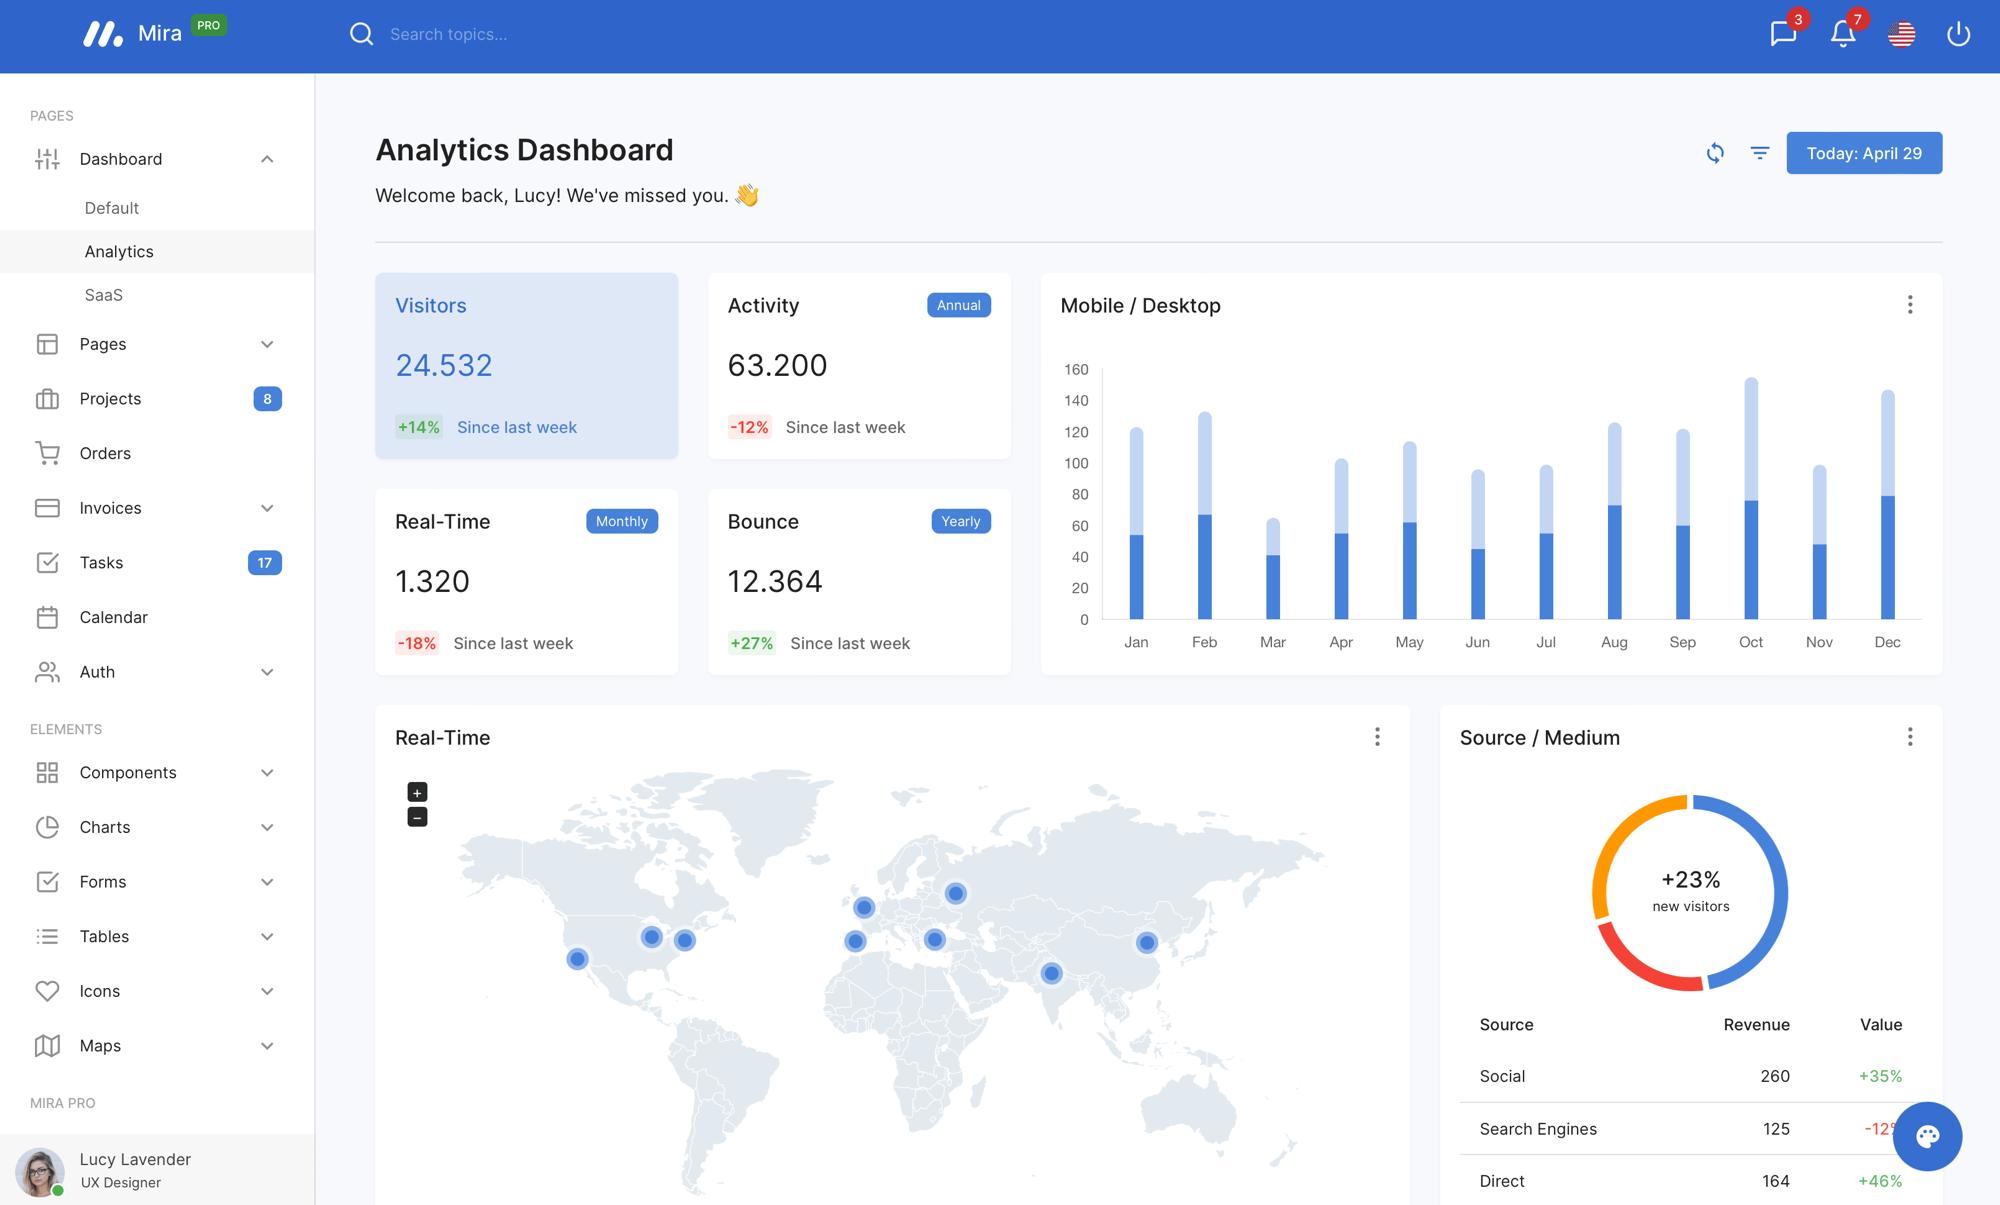
\includegraphics[width=0.90\textwidth,height=0.45\textheight,keepaspectratio]{imgs/mui_dashboard.png}
\fonte{Material UI. Disponível em: https://mui.com/. Acesso em: maio 2026.}
\end{figure}

Uma das vantagens do \textit{MUI} é a possibilidade de personalização por meio de temas. No projeto desenvolvido durante o estágio, foi criado um tema personalizado que definia as cores, tipografia e espaçamentos de acordo com a identidade visual da empresa cliente. Dessa forma, todos os componentes da biblioteca adotavam automaticamente o padrão visual definido, garantindo consistência em toda a plataforma.

Além dos componentes básicos do \textit{MUI}, o projeto utilizou a biblioteca \textit{MUI X Date Pickers} para os campos de seleção de data, recurso frequentemente utilizado nos formulários de protocolos que exigiam o registro de datas de plantio, colheita e emergência. Também foi utilizada a biblioteca \textit{TanStack React Table} para a construção de tabelas com funcionalidades avançadas de ordenação, paginação e filtragem.

\subsection{Visualização de Dados com ApexCharts}

A geração de gráficos e visualizações de dados constituiu o principal diferencial da plataforma em relação ao uso de planilhas. Para essa funcionalidade, foi utilizada a biblioteca \textit{ApexCharts}, uma biblioteca \textit{JavaScript} de código aberto para a criação de gráficos interativos. A integração com o \textit{React} foi realizada por meio do pacote \textit{react-apexcharts} \cite{ApexCharts2024}.

O \textit{ApexCharts} oferece diversos tipos de gráficos, como barras, linhas, pizza, radar e área, além de funcionalidades como \textit{zoom}, \textit{tooltip} e exportação em formato de imagem. Na plataforma de protocolos, foram utilizados principalmente gráficos de barras verticais e horizontais para comparar os resultados entre diferentes tratamentos e momentos de avaliação. O \autoref{cod:apexex} apresenta um exemplo didático da configuração mínima de um gráfico de barras com o pacote \textit{react-apexcharts}.

\begin{lstlisting}[caption={Exemplo didático de gráfico de barras com \textit{react-apexcharts}.}, label={cod:apexex}]
import ApexCharts from "react-apexcharts";

const series = [{ name: "Vendas", data: [10, 20, 30] }];
const options = {
  chart: { type: "bar" },
  xaxis: { categories: ["Jan", "Fev", "Mar"] },
};

export function GraficoVendas() {
  return <ApexCharts options={options} series={series} type="bar" />;
}
\end{lstlisting}

No exemplo, \texttt{series} é a lista de séries do gráfico, cada uma contendo um nome e um vetor de valores numéricos correspondentes a cada categoria. O objeto \texttt{options} concentra a configuração visual, definindo o tipo de gráfico (\texttt{chart.type}) e os rótulos do eixo horizontal (\texttt{xaxis.categories}). O componente \texttt{ApexCharts} recebe esses dois objetos e cuida da renderização do gráfico na tela.

\novop{A \autoref{fig:apexex} apresenta uma representação aproximada do gráfico produzido pelo \autoref{cod:apexex}, em que as três categorias (Jan, Fev e Mar) são exibidas no eixo horizontal e os valores numéricos correspondentes (10, 20 e 30) compõem as barras verticais.}

\begin{figure}[!htb]
\centering
\caption{\novo{Renderização aproximada do gráfico de barras configurado no \autoref{cod:apexex}.}}
\label{fig:apexex}
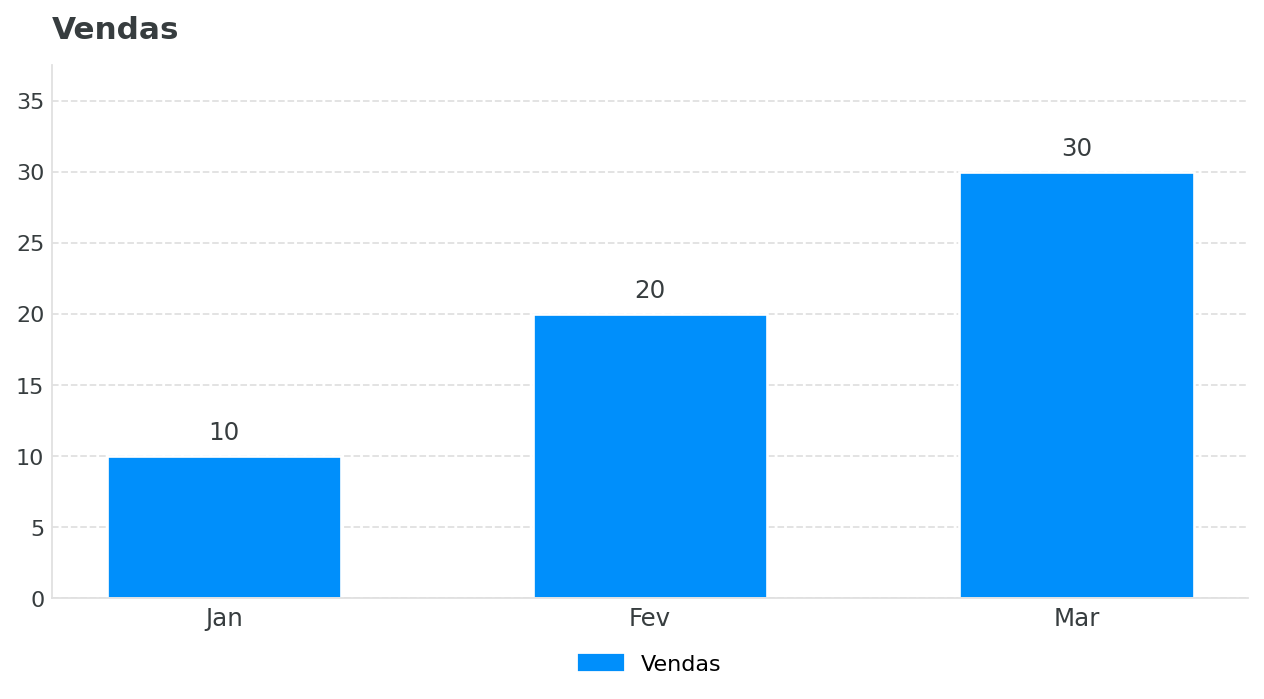
\includegraphics[width=0.65\textwidth,height=0.30\textheight,keepaspectratio]{imgs/apexcharts_vendas.png}
\fonte{\novo{do autor (2026), com base na biblioteca \textit{ApexCharts}.}}
\end{figure}

Para a avaliação de campos definidos como fórmulas nos protocolos, isto é, expressões matemáticas calculadas a partir dos valores de outros campos, foi utilizada a biblioteca \textit{mathjs}, que interpreta e avalia expressões em tempo de execução. A exportação dos gráficos em formato de imagem, com a identidade visual da empresa cliente, foi implementada com a biblioteca \textit{use-react-screenshot}, que captura um elemento da interface como imagem. Já a biblioteca \textit{JSZip} foi empregada para empacotar as fotografias de campo de uma avaliação em um único arquivo compactado para \textit{download}.

\chapter{\MakeUppercase{Metodologia e Processo de Desenvolvimento}}

Neste capítulo é descrito o processo de desenvolvimento adotado ao longo do estágio, abrangendo a aplicação da metodologia ágil \textit{Scrum}, o levantamento de requisitos e regras de negócio junto à empresa cliente e a arquitetura do \textit{front-end} construído. Para ilustrar as soluções tecnológicas, são apresentados, ao longo do texto, diagramas de alto nível e trechos simplificados do código desenvolvido, com a remoção de detalhes de estilo e de tratamento de erros para favorecer a legibilidade.

\section{Aplicação do \textit{Scrum} no Projeto}

O desenvolvimento da plataforma seguiu a metodologia \textit{Scrum}, organizada em \textit{Sprints} de duração fixa de duas semanas. No início de cada \textit{Sprint}, era realizada a reunião de \textit{planning}, na qual as tarefas priorizadas do \textit{Product Backlog} eram selecionadas e detalhadas no \textit{Sprint Backlog}. As tarefas eram acompanhadas em um quadro de tarefas dividido nas colunas de afazeres, em andamento, em revisão e concluído.

Para o gerenciamento do \textit{Product Backlog} e do \textit{Sprint Backlog} foi utilizado o \textit{Azure DevOps Boards}, ferramenta da \textit{Microsoft} voltada à gestão ágil de trabalho e ao acompanhamento de \textit{itens de trabalho} (\textit{Work Items}) ao longo do ciclo de desenvolvimento. Cada tarefa do \textit{backlog} possuía identificador, estado (por exemplo, \textit{New}, \textit{Approved} ou \textit{Committed}), título, área de produto e marcadores associados, o que facilitava a priorização e a distribuição das atividades entre os membros da equipe. A \autoref{fig:azure} apresenta um exemplo de tela do \textit{Azure DevOps Boards} com a listagem de \textit{Work Items} de um \textit{backlog}.

\begin{figure}[!htb]
\centering
\caption{Tela de \textit{backlog} do \textit{Azure DevOps Boards}.}
\label{fig:azure}
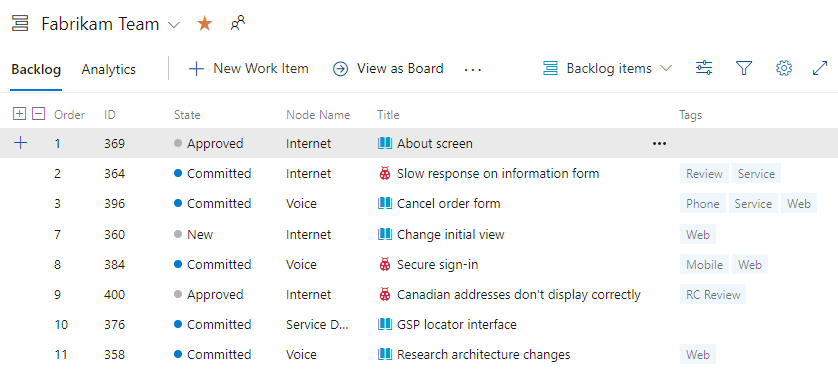
\includegraphics[width=0.95\textwidth,height=0.35\textheight,keepaspectratio]{imgs/azure_devops_backlog.png}
\fonte{Microsoft Learn. Disponível em: https://learn.microsoft.com/pt-br/azure/devops/boards/backlogs/create-your-backlog. Acesso em: maio 2026.}
\end{figure}

O acompanhamento diário ocorria por meio das \textit{daily meetings}, reuniões breves em que cada membro relatava o progresso, os planos do dia e eventuais impedimentos. Ao final de cada \textit{Sprint}, a \textit{Sprint Review} apresentava o incremento desenvolvido ao cliente, e a \textit{Sprint Retrospective} permitia à equipe refletir sobre o processo. A adoção desse fluxo possibilitou entregas incrementais à \novo{empresa cliente} e a validação contínua das funcionalidades, reduzindo o risco de retrabalho.

\section{Levantamento de Requisitos e Regras de Negócio}

O levantamento de requisitos foi conduzido de forma iterativa, em conjunto com a equipe da \novo{empresa cliente}. Como a empresa atua na pesquisa agrícola, muitas das regras de negócio eram específicas do domínio e não estavam formalmente documentadas, o que exigiu reuniões frequentes para esclarecer o comportamento esperado da plataforma.

\novop{O conjunto de regras que concentrou a maior complexidade foi o das regras de preenchimento dos protocolos, em que a obrigatoriedade e o formato de diversos campos dependiam do tipo de protocolo, da cultura selecionada e da classe do experimento. Como essas combinações não estavam descritas em nenhum documento, cada variação precisava ser esclarecida diretamente com a equipe do cliente antes de ser traduzida para o esquema de validação do formulário. Esses requisitos foram refinados a cada \textit{Sprint}, à medida que as telas eram apresentadas e validadas pelo cliente.}

\section{Arquitetura do \textit{Front-end} e Estrutura do Projeto}

A aplicação foi construída como uma \textit{Single Page Application} (SPA) em \textit{React} com \textit{TypeScript}, empacotada pelo \textit{Vite}. A organização do código seguiu uma separação por responsabilidades, distribuída em três camadas lógicas: a camada de apresentação, responsável pela renderização da interface; a camada de estado, responsável por manter os dados em memória durante a navegação; e a camada de acesso a dados, responsável pela comunicação com a API do servidor. A \autoref{fig:arquitetura} apresenta uma visão de alto nível dessa organização.

\begin{figure}[!htb]
\centering
\caption{Arquitetura em camadas do \textit{front-end} da plataforma de protocolos.}
\label{fig:arquitetura}
\vspace{0.3cm}

\begin{tikzpicture}[
  node distance=0.7cm,
  layer/.style={rectangle, draw, rounded corners, align=center,
                text width=11cm, minimum height=1.1cm, fill=gray!8},
  ext/.style={rectangle, draw, rounded corners, align=center,
              text width=7cm, minimum height=1cm, fill=gray!20},
  seta/.style={-{Latex}, thick}
]
\node[layer] (apres) {\textbf{Camada de Apresentação}\\ Componentes \textit{React}, \textit{Material UI}, \textit{TanStack Table} e \textit{ApexCharts}};
\node[layer, below=of apres] (estado) {\textbf{Camada de Estado}\\ \textit{Zustand} (estado global) e \textit{Formik} + \textit{Yup} (formulários)};
\node[layer, below=of estado] (dados) {\textbf{Camada de Acesso a Dados}\\ Camada de serviços sobre o \textit{Axios} (injeção de \textit{token} e \textit{refresh token}) e \textit{React Query} (\textit{cache} e sincronização)};
\node[ext, below=of dados] (api) {\textbf{API REST} (\textit{back-end})};
\draw[seta] (apres) -- (estado);
\draw[seta] (estado) -- (dados);
\draw[{Latex}-{Latex}, thick] (dados) -- (api);
\end{tikzpicture}

\vspace{0.2cm}
{\footnotesize Fonte: do autor (2026).}
\end{figure}

\novop{É importante destacar que o \textit{back-end} da plataforma, incluindo a API REST representada na \autoref{fig:arquitetura}, não foi desenvolvido pelo autor deste trabalho. Sua construção ficou a cargo de outra equipe da Zeeway, dedicada exclusivamente ao desenvolvimento do servidor, da modelagem do banco de dados e da implementação das regras de negócio do lado do servidor. Os capítulos seguintes detalham apenas as atividades realizadas na camada de \textit{front-end}.}

\novop{A coordenação entre as duas equipes foi baseada em uma estratégia de paralelização do trabalho a partir de uma interface comum. No início de cada nova funcionalidade, eram definidos em conjunto os contratos das chamadas à API, isto é, o caminho de cada \textit{endpoint}, o método HTTP utilizado e a estrutura dos dados de entrada e de saída. Com esse contrato acordado, as duas equipes passavam a trabalhar simultaneamente na mesma \textit{Sprint}: a equipe de \textit{back-end} implementava o \textit{endpoint} correspondente, enquanto a equipe de \textit{front-end} construía a tela e consumia inicialmente os dados em uma versão mascarada (\textit{mock}) que respeitava o contrato. Quando o \textit{endpoint} ficava disponível, a integração era feita substituindo a fonte dos dados pela API real. Ajustes pontuais no contrato eram negociados nas reuniões diárias ou na \textit{planning} da \textit{Sprint} seguinte, evitando que uma equipe ficasse permanentemente em ritmo diferente da outra.}

A estrutura de diretórios do projeto refletia essa separação de responsabilidades, agrupando os arquivos por função, conforme ilustrado no \autoref{cod:estrutura}. Os diretórios \texttt{components/}, \texttt{pages/} e \texttt{layouts/} concentram a parte visual da aplicação, enquanto \texttt{store/}, \texttt{services/} e \texttt{routes/} tratam, respectivamente, do estado global, da comunicação com a API e da definição das rotas. O diretório \texttt{hooks/} centraliza os \textit{hooks} customizados, como \texttt{useForm} e \texttt{useRoles}, e \texttt{utils/} reúne funções auxiliares reutilizadas em diferentes contextos.

\begin{lstlisting}[caption={Organização simplificada dos diretórios do projeto.}, label={cod:estrutura}, numbers=none]
src/
  components/   Componentes reutilizaveis (tabelas, modais, graficos)
  config/       Constantes e configuracoes globais
  contexts/     Contextos de React
  hooks/        Hooks customizados (useForm, useRoles, React Query)
  layouts/      Layouts de pagina (autenticacao e listagem)
  pages/        Telas (Login, Protocols, Dashboard, Clients, ...)
  routes/       Definicao e guarda de rotas
  services/     Camada de servicos e chamadas a API (Axios)
  store/        Estado global (Zustand)
  theme/        Tema do Material UI
  types/        Tipos TypeScript compartilhados
  utils/        Funcoes auxiliares (axios, arquivos, debounce)
\end{lstlisting}

Na camada de acesso a dados, todas as chamadas à API passavam por uma função de serviço (\texttt{httpRequest}) que anexava automaticamente o \textit{token} de acesso do usuário autenticado ao cabeçalho de autorização, evitando a repetição dessa lógica em cada requisição. Além disso, foi configurado um interceptador de resposta do \textit{Axios} responsável por renovar o \textit{token} de forma transparente sempre que a API retornava o código de erro 401, reenviando a requisição original com o novo \textit{token} obtido a partir do \textit{refresh token}. O \autoref{cod:interceptor} apresenta um trecho simplificado dessa configuração.

\begin{lstlisting}[caption={Trecho do interceptador de resposta para renovação do \textit{token} (\textit{refresh token}).}, label={cod:interceptor}]
axiosInstance.interceptors.response.use(
  (response) => response,
  async (error) => {
    const originalRequest = error.config;
    if (error.response?.status === 401 && !originalRequest._retry) {
      const { refreshToken } = loginStorePersist.getState().session;
      originalRequest._retry = true;
      const response = await axiosInstance.post("/user/refreshToken", {
        refreshToken,
      });
      const newToken = response.data.data.accessToken;
      loginStorePersist.getState().setLoginInfo({ data: response.data });
      originalRequest.headers["Authorization"] = `Bearer ${newToken}`;
      return axiosInstance(originalRequest);
    }
    return Promise.reject(error);
  }
);
\end{lstlisting}

O trecho registra um interceptador para todas as respostas do \textit{Axios}. A primeira função do par recebe as respostas bem-sucedidas e as devolve sem alteração. A segunda função trata os erros: ela inspeciona o código HTTP retornado e só age quando este é 401 (não autorizado) e quando a requisição original ainda não foi reexecutada, controle feito pela marcação \texttt{\_retry}. Nessa situação, o \textit{refresh token} é obtido do \textit{store} de autenticação e enviado em uma nova requisição ao \textit{endpoint} \texttt{/user/refreshToken}; quando essa requisição é bem-sucedida, o novo \textit{access token} é gravado no \textit{store} por meio de \texttt{setLoginInfo}, o cabeçalho de autorização da requisição original é atualizado e ela é reenviada de forma transparente para o usuário. Em qualquer outro caso, o erro é propagado normalmente.

\chapter{\MakeUppercase{Resultados: A Plataforma de Protocolos}}

Neste capítulo são descritas as principais funcionalidades desenvolvidas durante o estágio para a plataforma de protocolos da Terra Gerais. A apresentação está organizada por módulo, detalhando as decisões técnicas tomadas e os desafios enfrentados em cada etapa. A seleção das atividades se deu por meio da sua relevância no escopo do projeto e pela complexidade técnica envolvida.

\section{Módulo de Autenticação e Controle de Acesso}

O primeiro módulo desenvolvido foi o de autenticação, responsável por controlar o acesso dos colaboradores da Terra Gerais à plataforma. A tela de login foi construída seguindo a identidade visual da empresa cliente, com campos para e-mail e senha e a opção de recuperação de senha.

A autenticação foi implementada com o uso da biblioteca \textit{jwt-decode} para decodificação de tokens JWT (\textit{JSON Web Token}) recebidos da API. Após o login bem-sucedido, os dados da sessão (\textit{access token} e \textit{refresh token}) e as informações do usuário extraídas do \textit{token} eram armazenados no estado global da aplicação, gerenciado pela biblioteca \textit{Zustand} com o \textit{middleware} de persistência. A atualização imutável desse estado foi feita com o auxílio da biblioteca \textit{Immer}. O \autoref{cod:store} apresenta um trecho simplificado da função que processa o login, decodificando o \textit{token} e populando o \textit{store}.

\begin{lstlisting}[caption={Trecho do \textit{store} de autenticação (\textit{Zustand}) com \textit{Immer} e \textit{jwt-decode}.}, label={cod:store}]
export const loginStorePersist = create(
  persist((set, get) => ({
    // ...estado inicial omitido
    setLoginInfo: ({ data }) =>
      set(produce((draft) => {
        draft.isAuthenticated = true;
        draft.session = {
          accessToken: data.data.accessToken,
          refreshToken: data.data.refreshToken,
        };
        const decoded = jwtDecode(data.data.accessToken);
        draft.userData = {
          name: decoded.unique_name,
          id: decoded.nameid,
          email: decoded.email,
          roleId: decoded.role,
        };
      })),
  }), { name: "UserData" })
);
\end{lstlisting}

O \textit{store} é criado com a função \texttt{create} do \textit{Zustand} combinada ao \textit{middleware} \texttt{persist}, que salva o conteúdo em armazenamento local sob o nome \texttt{UserData}, mantendo a sessão entre acessos. A função \texttt{setLoginInfo} é a operação central: ela é executada após o sucesso do login e recebe os dados retornados pela API. A chamada \texttt{produce}, do \textit{Immer}, expõe um \textit{draft} mutável do estado e permite escrever as alterações de forma direta. No bloco interno, o usuário é marcado como autenticado, os \textit{tokens} são gravados na sessão, o \textit{access token} é decodificado por \texttt{jwtDecode} e os campos relevantes (nome, identificador, e-mail e perfil) são extraídos das suas \textit{claims} e atribuídos a \texttt{userData}.

Um dos desafios deste módulo foi a implementação do controle de permissões por perfil de usuário. A plataforma previa dois perfis principais, Administrador e Técnico, com diferentes níveis de acesso às funcionalidades. O perfil Administrador possuía acesso completo ao sistema, incluindo a gestão de usuários, enquanto o perfil Técnico tinha acesso restrito apenas ao registro e consulta de protocolos. O controle foi implementado no nível das rotas, por meio de um componente guardião (\texttt{ProtectedRouteGuard}) que verificava, a partir do perfil armazenado no \textit{store}, se o usuário estava autenticado e se possuía permissão de administrador, redirecionando-o quando necessário. O \autoref{cod:permissao} apresenta um trecho desse componente.

\begin{lstlisting}[caption={Trecho do componente de guarda de rotas por perfil de usuário.}, label={cod:permissao}]
const ProtectedRouteGuard = ({ children, adminRoute }) => {
  const { isAuthenticated, userData: { roleId } } =
    loginStorePersist((state) => state);
  const { isUserRole } = useRoles();

  if (!isAuthenticated) {
    return <Navigate to="/login" replace />;
  }
  if (adminRoute && !isUserRole("administrador", roleId)) {
    return <Navigate to="/" replace />;
  }
  return children;
};
\end{lstlisting}

O componente recebe como propriedades os elementos filhos (\texttt{children}) que ele encapsula e a marcação \texttt{adminRoute}, usada para indicar rotas restritas ao administrador. As primeiras linhas leem do \textit{store} o estado de autenticação e o identificador do perfil do usuário, e obtêm do \textit{hook} \texttt{useRoles} a função utilitária \texttt{isUserRole}. Em seguida, duas verificações são feitas: a primeira garante que o usuário esteja autenticado, redirecionando-o para \texttt{/login} quando não estiver; a segunda só se aplica às rotas marcadas como \texttt{adminRoute} e redireciona para a raiz quando o perfil do usuário não é administrador. Quando nenhuma das condições dispara redirecionamento, os filhos são renderizados normalmente.

\subsection{Gestão de Usuários}

A tela de gestão de usuários permitia ao administrador visualizar, adicionar, editar e excluir os colaboradores cadastrados. A listagem exibia nome, tipo de perfil, e-mail e contato de cada usuário, com suporte a busca textual e filtros por tipo de perfil.

As operações de criação e exclusão de usuários eram realizadas por meio de modais, componentes sobrepostos à tela principal que permitem ao usuário executar uma ação sem perder o contexto da página atual. Foram implementados modais para o formulário de adição de usuário, para a confirmação de exclusão e para o \textit{feedback} de sucesso e erro. Todos os formulários utilizavam a biblioteca \textit{Formik} para gerenciamento de estado dos campos e \textit{Yup} para validação dos dados antes do envio à API.

\section{Módulo de Registros Agrícolas}

O módulo de registros agrícolas constituiu o núcleo da plataforma, sendo responsável pelo cadastro, edição e consulta dos protocolos de pesquisa. Cada protocolo representava um registro completo de uma pesquisa agrícola, contendo informações sobre a safra analisada, os tratamentos aplicados, as características do solo e os resultados de produtividade.

\subsection{Listagem de Protocolos}

A tela de listagem de protocolos foi construída utilizando a biblioteca \textit{TanStack React Table}, que oferece recursos avançados de tabela como ordenação, paginação e filtragem. Cada protocolo era exibido com seu código, tipo, cliente, classe, cultura e status atual. As ações disponíveis incluíam edição, exclusão, geração de QR Code e exportação para planilha.

A funcionalidade de geração de QR Code foi implementada com a biblioteca \textit{qrcode} e tinha como objetivo facilitar a identificação dos protocolos em campo. Cada QR Code gerado continha um identificador único que, ao ser escaneado, direcionava o colaborador diretamente para a página do protocolo correspondente na plataforma.

\subsection{Formulário de Cadastro e Edição de Protocolos}

O formulário de cadastro de protocolos representou um dos maiores desafios técnicos do projeto, dado o grande volume de campos e a complexidade das regras de negócio envolvidas. O formulário foi organizado em abas para melhorar a usabilidade: Informações, Avaliações, Tratamentos, Local, Solo, Aplicações, Manejo e Dashboard.

A aba de Informações continha os dados gerais do protocolo. Entre os campos obrigatórios estavam o tipo do protocolo (Ret ou Comercial), o código, o cliente, as classes do experimento, o status, o número de tratamentos e o número de repetições. Os demais campos eram opcionais, como cultura utilizada, variedade, cultura anterior, tipo de plantio, datas de plantio, colheita e emergência, adubação, espaçamento entre linhas, delineamento experimental, tamanho da parcela e parcela útil. Essa distinção entre campos obrigatórios e opcionais era expressa no esquema de validação apresentado adiante, e o campo de classes permitia a seleção de múltiplos valores, com a possibilidade de cadastrar novas classes diretamente no formulário.

A aba de Avaliações permitia o registro dos dados coletados em cada momento de avaliação. A estrutura desta aba era dinâmica: o número de colunas da tabela variava de acordo com o número de repetições configurado na aba de Informações, e novas linhas podiam ser adicionadas conforme a necessidade. Alguns campos podiam ser definidos como fórmulas, isto é, expressões matemáticas calculadas a partir dos valores de outros campos; para avaliar essas expressões em tempo de execução, foi utilizada a função \texttt{evaluate} da biblioteca \textit{mathjs}.

Além dos dados numéricos, a aba suportava o \textit{upload} de fotografias de campo, permitindo que os técnicos anexassem registros visuais diretamente vinculados a cada momento de avaliação. Para facilitar o trabalho posterior, foi implementada a funcionalidade de \textit{download} de todas as fotografias de uma avaliação em um único arquivo compactado, utilizando a biblioteca \textit{JSZip}. As imagens eram obtidas da API por meio de uma requisição gerenciada pelo \textit{React Query}, convertidas em \textit{blobs}, agrupadas em um arquivo \textit{.zip} e salvas no dispositivo do usuário, conforme o \autoref{cod:jszip}.

\begin{lstlisting}[caption={Trecho do \textit{download} das fotografias de uma avaliação em arquivo \textit{.zip} com \textit{JSZip}.}, label={cod:jszip}]
const handleDownloadImages = async (evaluation) => {
  getImages(evaluation.id, {
    onSuccess: async ({ data }) => {
      const images = data.data;
      const blobs = await Promise.all(
        images.map((img) => fetch(img.url).then((res) => res.blob()))
      );
      const zip = new JSZip();
      blobs.forEach((blob, i) => zip.file(`${images[i].title}.jpg`, blob));
      const zipFile = await zip.generateAsync({ type: "blob" });
      saveFile(zipFile, evaluation.name);
    },
  });
};
\end{lstlisting}

A função recebe a avaliação selecionada e dispara a busca das imagens pela API por meio do \textit{mutation} \texttt{getImages}, fornecido pelo \textit{React Query}. No \textit{callback} de sucesso, a lista de imagens retornada é percorrida e cada item é mapeado para uma promessa que baixa o arquivo como \textit{blob}, utilizando o \texttt{fetch} nativo do navegador; as promessas são aguardadas em paralelo com \texttt{Promise.all}. Em seguida, uma instância de \texttt{JSZip} é criada e cada \textit{blob} é adicionado ao arquivo com o nome correspondente. Por fim, o método \texttt{generateAsync} produz o arquivo \texttt{.zip} final em memória, que é entregue ao usuário pela função utilitária \texttt{saveFile}.

O gerenciamento do estado do formulário foi implementado com a biblioteca \textit{Formik}, encapsulada em um \textit{hook} customizado (\texttt{useForm}) que padronizava o controle dos valores dos campos e a orquestração das validações em todas as telas. Essa padronização era importante, dado que um protocolo podia conter dezenas de tratamentos, cada um com múltiplas repetições e avaliações, resultando em estruturas de dados profundamente aninhadas.

Uma das principais dificuldades encontradas neste módulo foi a tradução das regras de negócio da Terra Gerais para a lógica do formulário. As regras variavam conforme o tipo de protocolo, a cultura selecionada e a classe do experimento, exigindo uma comunicação constante com a equipe do cliente para validar o comportamento esperado. O uso da biblioteca \textit{Yup} para a definição de esquemas de validação mostrou-se essencial para garantir a integridade dos dados antes do envio ao servidor, distinguindo os campos obrigatórios dos opcionais e validando tipos, listas e formatos. O \autoref{cod:yup} apresenta um trecho do esquema de validação da aba de Informações do protocolo.

\begin{lstlisting}[caption={Trecho do esquema de validação (\textit{Yup}) da aba de Informações do protocolo.}, label={cod:yup}]
const validationSchema = Yup.object().shape({
  isRET: Yup.bool().required("O campo e obrigatorio"),
  code: Yup.string().required("O campo e obrigatorio"),
  culture: Yup.string(),
  experimentalDesign: Yup.string().nullable(),
  numberOfTreatments: Yup.number().required("O campo e obrigatorio").nullable(),
  numberOfRepeats: Yup.number().required("O campo e obrigatorio").nullable(),
  plantingDate: Yup.string().nullable(),
  harvestDate: Yup.string().nullable(),
  classes: Yup.array().min(1, "O campo e obrigatorio"),
  clientId: Yup.string().required("O campo e obrigatorio"),
});
\end{lstlisting}

O esquema é declarado com \texttt{Yup.object().shape}, recebendo um objeto cujas chaves correspondem aos campos do formulário. Cada chave aciona uma cadeia de validações específica do seu tipo: os campos do tipo \textit{string} ou \textit{bool} usam \texttt{.required} quando são obrigatórios; os campos numéricos combinam \texttt{.required} com \texttt{.nullable}, o que permite manter o campo nulo durante o preenchimento parcial, mas exige o seu preenchimento no envio; o campo \texttt{classes} utiliza \texttt{array().min(1)} para garantir ao menos uma classe selecionada; e os campos puramente opcionais (como \texttt{culture}) aparecem sem \texttt{.required}. A mensagem passada a cada validação é o texto exibido ao usuário quando a regra é violada.

\section{Módulo de Análise e Dashboards}

O módulo de análise e dashboards representou o principal diferencial da plataforma em relação ao uso de planilhas. A proposta era transformar os dados brutos registrados nos protocolos em visualizações gráficas que auxiliassem os pesquisadores na tomada de decisões.

\subsection{Geração Automatizada de Gráficos}

A geração de gráficos foi implementada utilizando a biblioteca \textit{ApexCharts}, integrada ao React por meio do pacote \textit{react-apexcharts}. Os componentes de gráfico recebiam os dados já consolidados (rótulos do eixo horizontal e valores correspondentes) e montavam, de forma automática, as séries e as opções de configuração do \textit{ApexCharts}, sem a necessidade de ajuste manual por parte do usuário. Foram utilizados principalmente gráficos de barras verticais e horizontais para comparar os resultados entre diferentes tratamentos e categorias. Cada gráfico era renderizado individualmente em um \textit{card}, com a opção de \textit{download} individual.

O processo de transformação dos dados em visualizações seguia um fluxo bem definido, desde a obtenção dos dados até a exportação da imagem final, conforme apresentado na \autoref{fig:pipeline}.

\begin{figure}[ht]
\centering
\caption{Fluxo de geração de gráficos a partir dos dados de avaliação.}
\label{fig:pipeline}
\vspace{0.3cm}

\begin{tikzpicture}[
  node distance=0.45cm,
  etapa/.style={rectangle, draw, rounded corners, align=center,
                text width=2.3cm, minimum height=1.6cm, font=\footnotesize, fill=gray!8},
  seta/.style={-{Latex}, thick}
]
\node[etapa] (dados) {Dados do \textit{back-end} (Dashboard)};
\node[etapa, right=of dados] (calc) {Mapeamento para séries (\textit{xAxis} / \textit{yAxis})};
\node[etapa, right=of calc] (serie) {Opções do \textit{ApexCharts}};
\node[etapa, right=of serie] (render) {Renderização (\textit{react-apexcharts})};
\node[etapa, right=of render] (export) {Exportação PNG (\textit{use-react-screenshot})};
\draw[seta] (dados) -- (calc);
\draw[seta] (calc) -- (serie);
\draw[seta] (serie) -- (render);
\draw[seta] (render) -- (export);
\end{tikzpicture}

\vspace{0.2cm}
{\footnotesize Fonte: do autor (2026).}
\end{figure}

O ponto central desse fluxo era a montagem das séries e das opções do gráfico a partir dos vetores de rótulos (\texttt{xAxis}) e valores (\texttt{yAxis}) recebidos pelo componente. O \autoref{cod:serie} apresenta um trecho dessa configuração para um gráfico de colunas.

\begin{lstlisting}[caption={Trecho da configuração de séries e opções de um gráfico com \textit{react-apexcharts}.}, label={cod:serie}]
const series = [{ name: xAxisTitle, data: yAxis }];

const options: ApexOptions = {
  chart: { type: "bar", toolbar: { show: false } },
  plotOptions: { bar: { distributed: true } },
  dataLabels: { enabled: true },
  xaxis: { categories: xAxis },
  yaxis: { max: maxValue + 1 },
};

return <ApexCharts options={options} series={series} type="bar" />;
\end{lstlisting}

O vetor \texttt{series} contém uma única série de dados, com o rótulo informado pela propriedade \texttt{xAxisTitle} e o conjunto de valores em \texttt{yAxis}. O objeto \texttt{options}, tipado por \texttt{ApexOptions}, agrupa as configurações visuais do gráfico: \texttt{chart} define o tipo \texttt{bar} e oculta a barra de ferramentas padrão; \texttt{plotOptions} ativa a coloração distribuída por categoria; \texttt{dataLabels} habilita a exibição dos valores numéricos sobre as colunas; \texttt{xaxis} informa as categorias do eixo horizontal a partir do vetor \texttt{xAxis}; e \texttt{yaxis} ajusta o valor máximo do eixo vertical com base no valor máximo dos dados. A última linha entrega esses dois objetos ao componente \texttt{ApexCharts}, que cuida da renderização propriamente dita.

Uma funcionalidade importante foi a exportação dos gráficos em formato PNG com a identidade visual da Terra Gerais, contendo o logotipo da empresa e o título dos dados. Para isso, foi mantido um elemento oculto na tela contendo o gráfico acompanhado do logotipo, e a sua captura como imagem foi realizada com a biblioteca \textit{use-react-screenshot}. A imagem resultante era então disponibilizada para \textit{download} por meio da criação dinâmica de um \textit{link}, conforme o \autoref{cod:export}.

\begin{lstlisting}[caption={Trecho da exportação de um gráfico em PNG com \textit{use-react-screenshot}.}, label={cod:export}]
const [_, takeScreenshot] = useScreenshot();

const downloadChart = async (format) => {
  const imageBase64 = await takeScreenshot(imageRef.current);
  const link = document.createElement("a");
  link.href = imageBase64;
  link.download = `${imageTitle} - ${chartTitle}.${format}`;
  link.click();
};
\end{lstlisting}

A primeira linha obtém, do \textit{hook} \texttt{useScreenshot}, a função \texttt{takeScreenshot}, usada para gerar uma imagem a partir de um elemento do DOM. A função \texttt{downloadChart} é assíncrona e recebe como argumento o formato de imagem desejado. No seu corpo, \texttt{takeScreenshot} captura o elemento referenciado por \texttt{imageRef}, que contém o gráfico acompanhado do logotipo, devolvendo a imagem em \textit{base64}. Em seguida, um elemento de \textit{link} é criado dinamicamente, o atributo \texttt{href} recebe a imagem capturada, o atributo \texttt{download} define o nome do arquivo final (combinando o título da imagem, o título do gráfico e o formato) e o clique programático no \textit{link} força o navegador a salvar a imagem no dispositivo do usuário.

\subsection{Dashboard Geral}

Além dos gráficos individuais por protocolo, a plataforma contava com um dashboard geral que apresentava uma visão consolidada de todos os protocolos cadastrados, incluindo a distribuição de protocolos por classe, por cultura e por status.

Os dados consolidados desse dashboard, como a contagem e o percentual de protocolos por cultura, por classe e por cliente, eram fornecidos por um \textit{endpoint} específico do \textit{back-end} e buscados via API utilizando o \textit{React Query} (\textit{TanStack Query}), que gerenciava o cache das requisições e garantia que as visualizações estivessem sempre atualizadas sem a necessidade de recarregamentos manuais da página. No \textit{front-end}, esses dados eram mapeados para os vetores de rótulos e valores consumidos pelos componentes de gráfico.

Uma das dificuldades técnicas enfrentadas na construção dos dashboards foi a performance de renderização quando o volume de dados era elevado. A renderização simultânea de múltiplos gráficos com grandes conjuntos de dados causava lentidão perceptível na interface. Para mitigar esse problema, foi adotada uma estratégia de carregamento sob demanda (\textit{lazy loading}), em que os gráficos eram renderizados apenas quando o usuário navegava até a seção correspondente.

\chapter{\MakeUppercase{Considerações Finais}}\label{sec:conclusao}

Este capítulo apresenta uma avaliação do produto desenvolvido durante o estágio e uma reflexão sobre o impacto da experiência na formação acadêmica e profissional do autor. Retomam-se, de forma sintética, os objetivos definidos na introdução, discutindo em que medida foram alcançados e quais limitações e aprendizados foram observados ao longo do processo.

\section{Avaliação do Produto Desenvolvido}

O objetivo central do projeto era substituir o registro descentralizado de dados de pesquisa, antes mantido em planilhas eletrônicas, por uma plataforma web própria capaz de centralizar os protocolos da Terra Gerais, controlar o acesso por perfil de usuário e gerar análises visuais de forma automatizada. Diante das funcionalidades entregues, considera-se que esse objetivo foi atendido no plano técnico.

A camada de autenticação e o controle de acesso por perfil garantiram que cada colaborador interagisse apenas com as funcionalidades pertinentes ao seu papel, com renovação transparente de sessão por meio do mecanismo de \textit{refresh token}. O módulo de registros agrícolas implementou o cadastro completo dos protocolos, incluindo formulários extensos com validação declarativa e estruturas dinâmicas para as avaliações de campo. Por fim, o módulo de análise concretizou o principal diferencial da plataforma em relação às planilhas: a geração automatizada de gráficos e \textit{dashboards}, com exportação das visualizações em imagem padronizada pela identidade visual da empresa.

Entre as principais dificuldades superadas, destacam-se a tradução das regras de negócio do domínio agronômico para a lógica dos formulários, que exigiu validação contínua junto ao cliente, e a manutenção de um desempenho adequado na renderização simultânea de múltiplos gráficos, mitigada pela adoção de carregamento sob demanda. Como limitação, observou-se que a adoção da plataforma pelo cliente foi inicialmente reduzida, o que pode ser atribuído à mudança de cultura exigida pela transição das planilhas para um sistema estruturado, e não a uma deficiência técnica da solução. Trabalhos futuros poderiam incluir o acompanhamento dessa adoção ao longo do tempo, a realização de testes de usabilidade com os colaboradores e a evolução dos \textit{dashboards} com novos tipos de análise.

\section{Impacto do Estágio na Formação Acadêmica e Profissional}

O estágio representou a primeira experiência profissional do autor com o desenvolvimento de \textit{software} em um produto real, em equipe estruturada e com um cliente externo. Essa vivência permitiu aplicar, em um contexto concreto, conhecimentos adquiridos ao longo da graduação em disciplinas de engenharia de \textit{software}, desenvolvimento web, banco de dados e interação humano-computador, evidenciando como esses conteúdos se articulam na prática.

No plano técnico, a experiência consolidou competências em desenvolvimento \textit{front-end} com React e TypeScript, no uso de bibliotecas de interface e de gerenciamento de estado, na integração com APIs e, sobretudo, na visualização de dados por meio de gráficos e \textit{dashboards}, área que passou a orientar os interesses profissionais do autor. A adoção da metodologia Scrum proporcionou contato com o trabalho iterativo e incremental, com reuniões de planejamento e acompanhamento, e com a importância das entregas frequentes ao cliente.

No plano interpessoal, o estágio desenvolveu habilidades de comunicação e de trabalho em equipe, especialmente no levantamento de requisitos e na tradução de necessidades de negócio em soluções técnicas, atividade que exigiu diálogo constante com o cliente e com os demais membros da equipe. De modo geral, a experiência contribuiu de forma significativa para o amadurecimento profissional do autor e para a definição de um direcionamento de carreira voltado ao desenvolvimento de interfaces orientadas a dados, integrando a construção de aplicações web à análise e visualização de informações.


%==============================================================================
% Bibliografia

% Carrega o estilo para referências ABNT
\bibliographystyle{abntex2-alf}            

% Alterando informações do estilo de citação.
% Como estamos usando uma versão alterada, essas opções são necessárias.
% Et al. em itálico
\citeoption{abnt-etal-text=it}

% Até 3 autores antes do et al.
\citeoption{abnt-etal-cite=3}

% Colocar s.d. na falta de um ano de publicação
\citeoption{abnt-missing-year=sd}

% Altera o estilo de citação para (Autor, ano)
% A opção abnt-cite-style=AuthorYEAR está quebrada; essa é equivalente.
\citeoption{abnt-nbr10520=1988} 


% Comando necessário para corrigir o título das referências.
% Para o estilo ABNT, esse comando SEMPRE deve ser
% chamado antes do \bibliography
\referencias
% Adiciona as referência em bibtex 
\bibliography{refbib}

%==============================================================================
% Outros elementos pós-textuais

% Glossário (descomente se necessário)
%\glossario

% Anexos (descomente se necessário)
%\input{anexos/anexo1}

% Apêndices (descomente se necessário)
%\input{apendices/apendice1}

% Índice (descomente se necessário)
%\indice


%==============================================================================
% Fim do documento
%==============================================================================
\end{document}
